\section{Limitations and Future Work}

In this section, we discuss some limitations of our work and future research directions.
Because this is a new concept, it opens the door for many future research directions.
The first limitation is the color map that we use to depict the data in our cartograms. 
We use D3's built-in interpolateRdYlGn color map, a diverging color scheme of red, yellow, and green.
However, we believe that the choice of color map can have a significant impact on the legibility of cartograms.
In the user study, we carefully avoid extreme values where the location or color of the CCG makes it easier to locate the target.
See \Cref{fig:extreme} for an example.
We plan to explore the impact of different color maps on the legibility of cartograms in future work.

{
    \begin{figure}[tb!]
        \centering
        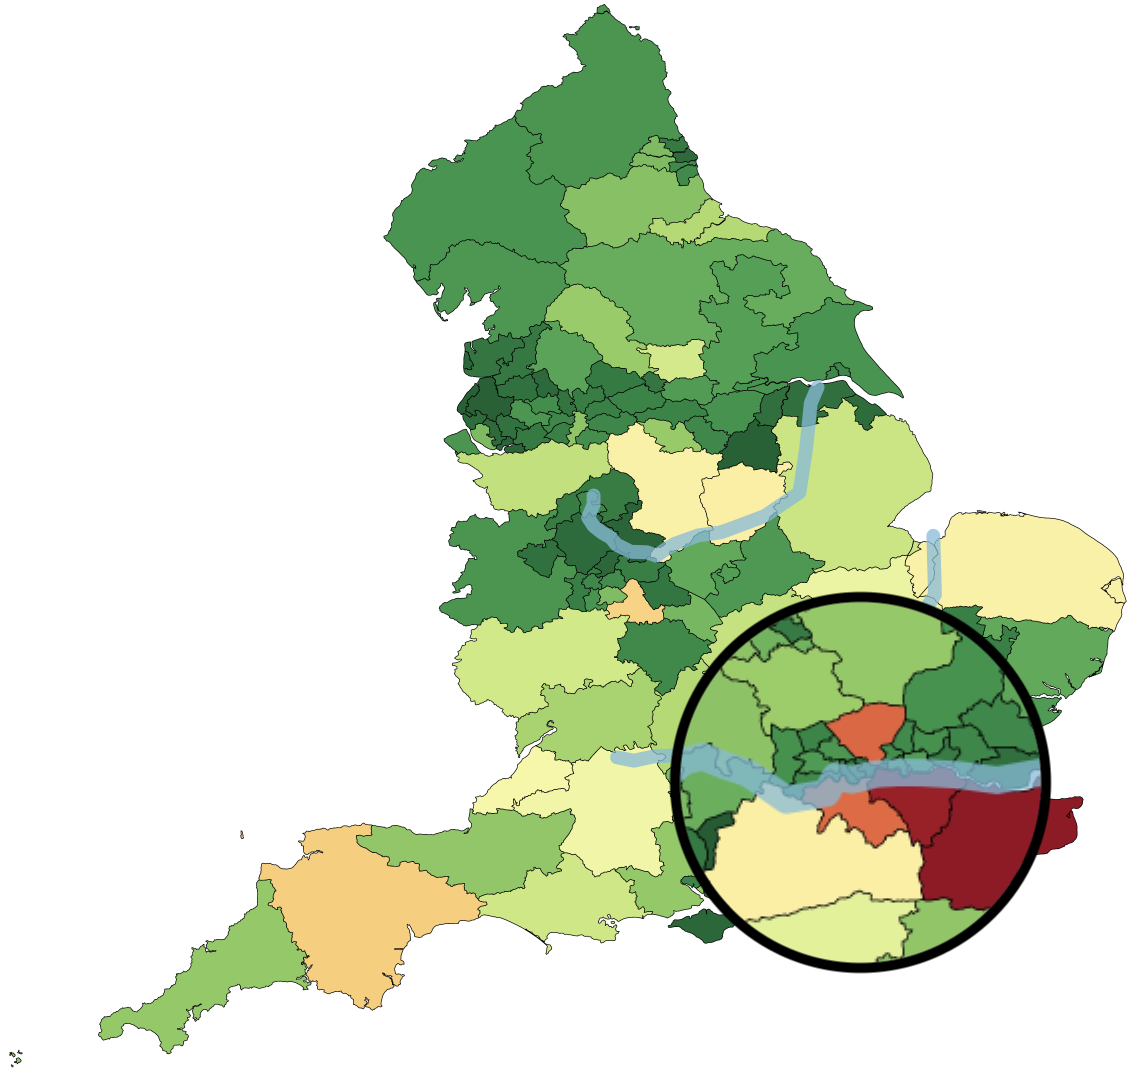
\includegraphics[width=0.7\columnwidth,keepaspectratio]{figure/limitations/extreme.png}
        \caption{Due to color and relative location, we believe the CCGs in the black circle are easier to locate.}
        \label{fig:extreme}
    \end{figure}
}

Another limitation is the overlap removal algorithm (FNOR) we use.
We believe that developing a new algorithm with built-in constraint support can significantly reduce the time required to generate cartograms with rivers. Currently, the runtime of our layout algorithm is approximately 30 milliseconds for each iteration.

Future work also includes generalizations and extensions of the algorithm, e.g., the use of other features in the cartogram layout such as additional rivers, major highways, lakes, and coastlines, etc.
We also consider whether increasing the length of the rivers as the size of the nodes increases would be a useful option.
We would like to explore the case of river-river intersections and testing out more geographies such as the U.S. and Europe, which have more complex rivers.
We also considered the idea of deforming the rivers as part of the layout algorithm, however, this idea is open to future work.
Furture work also includes adding rivers to dorling-style cartograms.
